\documentclass[8pt]{extarticle}
\title{}
\author{Avinash Iyer}
\date{}

%font setup
%
%\usepackage[math]{anttor}

%paper setup
\usepackage{geometry}
\geometry{letterpaper, portrait, margin=1in}
\usepackage{fancyhdr}

%symbols
\usepackage{amsmath}
\usepackage{amssymb}
\usepackage{hyperref}
\usepackage{gensymb}

\usepackage[T1]{fontenc}
\usepackage[utf8]{inputenc}

%chemistry stuff
\usepackage[version=4]{mhchem}
\usepackage{chemfig}

%plotting
\usepackage{pgfplots}
\usepackage{tikz}

%\usepackage{natbib}

%graphics stuff
\usepackage{graphicx}
\graphicspath{ {./images/} }

%a useful command
\newcommand{\plain}[1]{\textrm{#1}}

%code stuff
%when using minted, make sure to add the -shell-escape flag
%you can use lstlisting if you don't want to use minted
%\usepackage{minted}
%\usemintedstyle{pastie}
%\newminted[javacode]{java}{frame=lines,framesep=2mm,linenos=true,fontsize=\footnotesize,tabsize=3,autogobble,}
%\newminted[cppcode]{cpp}{frame=lines,framesep=2mm,linenos=true,fontsize=\footnotesize,tabsize=3,autogobble,}

\usepackage{listings}
\usepackage{color}
\definecolor{dkgreen}{rgb}{0,0.6,0}
\definecolor{gray}{rgb}{0.5,0.5,0.5}
\definecolor{mauve}{rgb}{0.58,0,0.82}

\lstset{frame=tb,
	language=Java,
	aboveskip=3mm,
	belowskip=3mm,
	showstringspaces=false,
	columns=flexible,
	basicstyle={\small\ttfamily},
	numbers=none,
	numberstyle=\tiny\color{gray},
	keywordstyle=\color{blue},
	commentstyle=\color{dkgreen},
	stringstyle=\color{mauve},
	breaklines=true,
	breakatwhitespace=true,
	tabsize=3
}
\pagestyle{fancy}
\fancyhf{}
\rhead{Avinash Iyer, Tobias Searcy-Jorgensen}
\lhead{Lab 4}
\begin{document}{
\section*{Part 1}
\begin{quote}
	First, make a quantitative prediction, i.e. calculate $ R_{\plain{theo}} $ and its uncertainty $ \delta R_{\plain{theo}} $ using equations [5] and [6].
\end{quote}
\subsection*{Subpart A}
\begin{quote}
	What measurements do you need to make in order to perform this calculation?  Report the best estimates for the measured quantities in the space below.
\end{quote}
We need a measurement of the height of the whole track and a measurement of the height of the bottom of the track, with instrumental uncertainty of 0.5 cm. We used the plumb bob to find the heights, and measured its length.
\begin{itemize}
	\item $H = h_1 + h_2 = 179.7\pm 0.5~\plain{cm}$ 
	\item $h_2 = 93.5\pm 0.5~\plain{cm}$ 
	\item $h_1 = 86.2\pm 0.5~\plain{cm}$
\end{itemize}
\subsection*{Subpart B}
The uncertainties in these measurements are primarily instrumental uncertainty — we solved the problem of definition by using the bottom edge of both the top of the track and the bottom of the track in order to standardize our measurement to the instrumental uncertainty.
\subsection*{Subpart C}
\begin{align*}
	R_{\plain{theo}} &= \sqrt{\frac{20}{7}h_1h_2} \\
	&=\boxed{1.52~\plain{m}} \\
	\delta R_{\plain{theo}} &= \sqrt{\frac{20}{7}} \times \frac{1}{2} \times \sqrt{\frac{h_2}{h_1}(\delta h_1)^2 + \frac{h_1}{h_2}(\delta h_2)^{2}} \\
	&= 0.60~\plain{m} \\
	R &= \boxed{1.52\pm 0.06~\plain{m}}
\end{align*}
\section*{Part 2}
\begin{quote}
	The goal of this experiment is to compare the theoretical prediction of the range, $ R_{\plain{theo}} $ from above, to the actual experimental range $ R{\plain{exp}} $.  Design an experiment that could test the theory as accurately as possible.  Use graph paper and carbon paper to record the ball’s landing position accurately. 
\end{quote}
\subsection*{Subpart A}
\begin{quote}
	Decide how you will experimentally measure the range R for each ball that is launched.  Choose the origin and the orientation of the coordinate system that you will use for data analysis.  Should the horizontal portion of the tube be considered in the measurements?  (Hint: At what point in the ball’s path does the projectile motion actually begin?)
\end{quote}
We will put graph paper on the floor around where the ball usually lands, calculate the $y$ distance from the point where the ball lands to the point where the ball leaves the tube, and average over those.
\subsection*{Subpart B}
\begin{quote}
	Assuming that friction in the tube is negligible, does anything happen to the ball’s speed or trajectory in the horizontal portion of the tube?
\end{quote}
There is no change to the speed of the ball or the trajectory of the ball while it is in the horizontal portion of the tube.
\subsection*{Subpart C}
\begin{quote}
	How accurately do you know the position of the initial launch point?  Decide how you can improve the accuracy of defining the initial launch point.  (Hint: A plumb bob is available.)
\end{quote}
We can find the launch point quite accurately by putting tape on the ground approximately below where the tube sits, drop a plumb bob with the string held against the launch point, and mark it on the tape, thereby finding an accurate launch point.
\section*{Part 3}
\begin{quote}
	Perform \textbf{5 trials}.  Place a ball in the upper end of the tube and simply release it — \textit{do not push it or spin it}.
\end{quote}
\subsection*{Subpart A}
\begin{quote}
	Record the x and y coordinates of each landing point in an Excel worksheet (although you really should include an uncertainty in your x and y measurements, for simplicity we are not asking you to do this here).  Then use the data (x and y) to calculate R for each data point. Use Excel formulas to do the calculations for you… do not waste time doing them all manually!  Include a data table with the x, y, and R values for each trial in the space below.  Show a sample calculation of R for one trial.
\end{quote}
\begin{center}
	\begin{tabular}{c|c|c}
		$x$ & $y$ & $R = 135 + y$ \\
		\hline
		-1.8 &	2.8 &	137.8 \\
		-1.6 &	-6.8 &	128.2 \\
		-3 &	-6.4 &	128.6 \\
		7.5 & 	-8.5 &	126.5 \\
		9.5 &	-4.4 &	130.6
	\end{tabular}
\end{center}
\subsection*{Subpart B}
\begin{quote}
	Determine the best estimate for the range $ R_{\plain{exp}} $ using Excel.
\end{quote}
The average of this set is $130.3$ cm, which is our $R_{\plain{exp}}$.
\subsection*{Subpart C}
\begin{quote}
	Determine the standard deviation (SD) $ \sigma_R $ of the R measurements using Excel.
\end{quote}
The standard deviation is $4.4$.
\subsection*{Subpart D}
\begin{quote}
	Calculate the standard deviation of the mean (SDOM) $ \sigma_{\overline{R}} $ of the set of $ R $ measurements.  This is the random uncertainty $ \delta R_{\plain{exp}} $ in the experimental value of the range. 
\end{quote}
The SDOM is $\frac{\sigma_{R}}{\sqrt{5}} = 1.9$.
\subsection*{Subpart E}
\begin{quote}
	Report the best estimate for the range and its uncertainty in an appropriate format ($ R_{\plain{exp}} \pm \delta R_{\plain{exp}} $).
\end{quote}
\[ R = 130.6\pm 1.9~\plain{cm} \]
\subsection*{Subpart F}
\begin{quote}
	Is the experimental result consistent with the theoretical prediction, considering uncertainties?
\end{quote}
No, the experimental result is well below the theoretical prediction, even considering the theoretical prediction's uncertainties.
\section*{Part 4}
\begin{quote}
	Now perform at least \textbf{40 trials}.
\end{quote}
\subsection*{Subpart A}
\begin{quote}
	Include your graph paper with the landing point distribution in the space below.  Does the scatter plot show what you expected to see?  Does it provide insight into the accuracy and the precision of your measurements?
\end{quote}
\begin{center}
	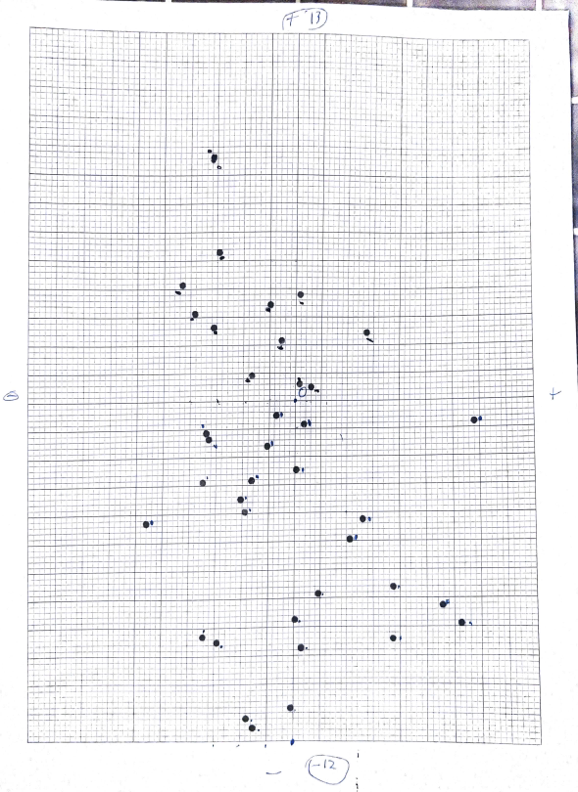
\includegraphics[width=15cm]{Lab3Image4_1}
\end{center}
The accuracy of our measurements is a little suspect, but all of our measurements were within a 18–20cm window. Meanwhile, the precision was within 2 millimeters.
\pagebreak 
\subsection*{Subpart B}
\begin{center}
	\begin{tabular}{c|c|c}
		$x$ & $y$ & $R = 132 + y$ \\
		\hline
		-0.2 &	-10.8 &	133.2 \\
		-1.6 &	-11.6 &	132.4 \\
		-1.8 &	-11.2 &	132.8 \\
		0.3 &	-8.7 &	135.3 \\
		-2.9 &	-8.5 &	135.5 \\
		0 & 	-7.8 &	136.2 \\
		-3.4 &	-8.3 &	135.7 \\
		1 & 	-6.8 & 	137.2 \\
		3.8 &	-8.4 &	135.6 \\
		3.8 &	-6.6 &	137.4 \\
		5.6 &	-7.2 &	136.8 \\
		6.2 &	-7.9 &	136.1 \\
		2.1 &	-5 &	139 \\
		6.8 &	-0.8 &	143.2 \\
		2.6 &	-4.3 &	139.7 \\
		0.1 &	-2.5 &	141.5 \\
		-1.9 &	-3.9 &	140.1 \\
		-2.1 &	-3.5 &	140.5 \\
		-1.7 &	-2.9 &	141.1 \\
		-3.5 &	-2.9 &	141.1 \\
		-5.6 &	-5.3 &	138.7 \\
		-0.7 &	-0.5 &	143.5 \\
		0.4 &	-0.8 &	143.2 \\
		-1.1 &	-1.6 &	142.4 \\
		-3.3 &	-1.2 &	142.8 \\
		-3.4 &	-1.1 &	142.9 \\
		0.2 &	2.8 &	146.8 \\
		0.2 &	0.6 &	144.6 \\
		0.6 &	0.5 &	144.5 \\
		0.7 &	0.9 &	144.9 \\
		0.5 &	2.2 &	146.2 \\
		-1 &	3.5 &	147.5 \\
		3.5 &	2.8 &	146.8 \\
		-3.1 &	2.6 &	146.6 \\
		3.8 &	3.1 &	147.1 \\
		-2.8 &	5.3 &	149.3 \\
		-4.3 &	4.1 &	148.1 \\
		3.2 &	8.5 &	152.5 \\
		3.2 &	8.6 &	152.6 \\
		2.4 &	-13 &	131 \\
	\end{tabular}
\end{center}
\subsection*{Subpart C}
\begin{quote}
	Determine the best estimate for the range $ R_{\plain{exp}} $.
\end{quote}
The best estimate for $R_{\plain{exp}}$ is $141.3$ cm.
\subsection*{Subpart D}
\begin{quote}
	Determine the standard deviation (SD) $ \sigma_R $ of the $ R $ measurements.
\end{quote}
The standard deviation of the $R$ measurements is $5.4$ cm.
\subsection*{Subpart E}
\begin{quote}
	Calculate the standard deviation of the mean (SDOM) $ \sigma_{\overline{R}} $ of the set of $ R $ measurements.
\end{quote}
The SDOM is $ \frac{\sigma_{R}}{\sqrt{40}}  = 0.9$
\subsection*{Part F}
\begin{quote}
	Report the best estimate for the range and its uncertainty in an appropriate format ($ R_{\plain{exp}} \pm \delta R_{\plain{exp}} $).
\end{quote}
\[ R = 141.3 \pm 0.9~\plain{cm} \]
\subsection*{Subpart G}
\begin{quote}
	Is the experimental result consistent with the theoretical prediction, considering uncertainties?  If not, discuss possible reasons.
\end{quote}
\begin{itemize}
	\item The experimental result is smaller than the theoretical prediction.
	\item The theory assumed zero friction, while of course there was a lot of friction with this setup from the ball clanging around inside the tube.
\end{itemize}
\section*{Conclusion}
\subsection*{Part 1}
\begin{quote}
	Compare the best estimates for the range from the two experiments – with a small and large numbers of trials.  Are they consistent with each other, considering experimental uncertainties?
\end{quote}
They are not consistent with each other even considering experimental uncertainties. This is likely because different people released the ball on each try.
\subsection*{Part 2}
\begin{quote}
	Compare the random uncertainty in the first experiment to the random uncertainty in the second experiment.  Describe how the number of trials affected the random uncertainty.
\end{quote}
The random uncertainty in the first trial was much larger than the random uncertainty in the second trial — because there were a much larger number of trials in the second trial, the standard deviation due to randomness was reduced significantly.
\subsection*{Part 3}
\begin{quote}
	Suppose you had a ruler, long enough to make direct measurements of the total distances traveled by the balls (eliminating the need for the coordinate system and separate x and y measurements).  Assuming that the smallest increment on this ruler is 1 mm (like the rulers/meter sticks used in class), would such a method improve the precision of the range measurements? Explain why or why not.
\end{quote}
Direct measurement of the range would not change the results because the random uncertainty was primarily from the idiosyncrasies in the way the ball was launched rather than the instrumental uncertainties of measurement.
}\end{document}
